
%***************************************************************************
%
% CreditCruncher - A portfolio credit risk valorator
% Copyright (C) 2004 Gerard Torrent
%
% This program is free software; you can redistribute it and/or
% modify it under the terms of the GNU General Public License
% as published by the Free Software Foundation; either version 2
% of the License.
%
% This program is distributed in the hope that it will be useful,
% but WITHOUT ANY WARRANTY; without even the implied warranty of
% MERCHANTABILITY or FITNESS FOR A PARTICULAR PURPOSE.  See the
% GNU General Public License for more details.
%
% You should have received a copy of the GNU General Public License
% along with this program; if not, write to the Free Software
% Foundation, Inc., 59 Temple Place - Suite 330, Boston, MA 02111-1307, USA.
%
%
% implementation.tex - TeX documentation file
% --------------------------------------------------------------------------
%
% 2005/01/22 - Gerard Torrent [gerard@fobos.generacio.com]
%   . initial release
%
%***************************************************************************

\chapter{Implementaci\'on de la soluci\'on}
\label{sec:implementation}

\section{Discretizaci\'on del problema}

Por motivos de rendimiento se selecciona un conjunto de nodos equiespaciados
en el eje temporal.

\subsection{Particionamiento del tiempo}

\begin{figure}[!hb]
\begin{center}
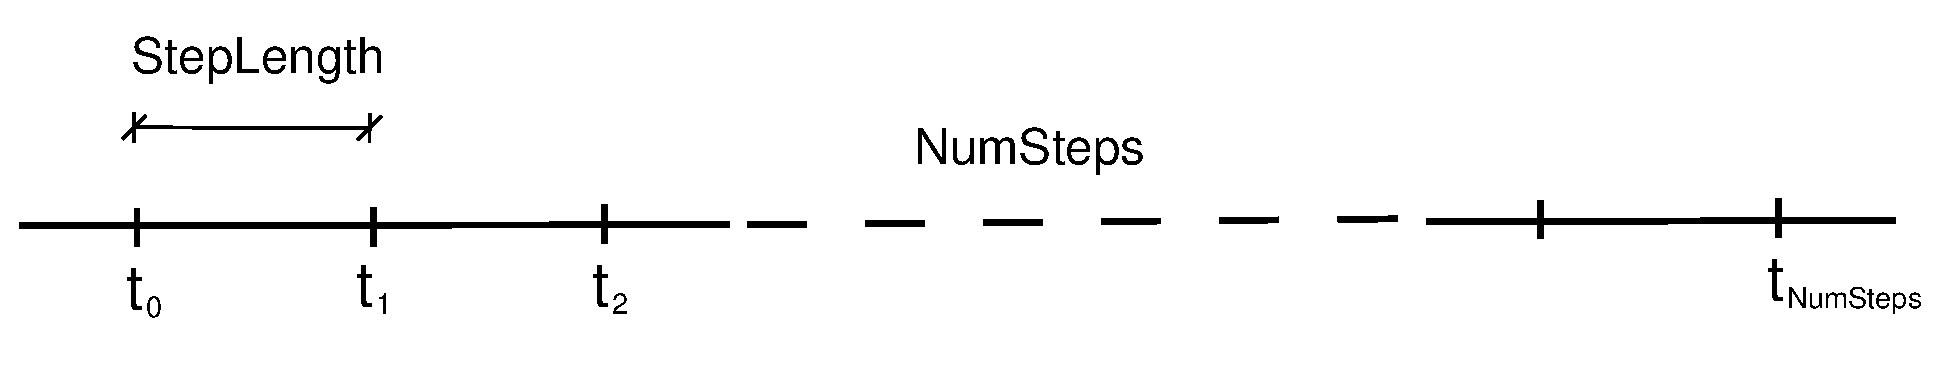
\includegraphics[width=10cm,angle=0]{./images/time.eps}
\caption{Particionamiento del tiempo}
\label{timetranches}
\end{center}
\end{figure}

\subsection{Mapeo del cashflow}

\subsection{Mapeo del netting}

\subsection{Ejemplo}

%---------------------------------------------------------------------------

\section{Interpretaci\'on del fichero de entrada}

El contenido esperado del fichero de entrada se encuentra
descrito en \emph{CreditCruncher - Input File Reference}
que se adjunta junto al programa.

El fichero de entrada puede tener un tama\~no considerable. Por
este motivo la lectura del fichero xml debe realizarse usando un
sistema orientado a eventos (tipo SAX). A continuaci\'on se
describen algunas de las validaciones que deben tenerse en cuenta:

\paragraph{Formato.} Se verifica que se trata de un fichero XML
v\'alido que cumple la DTD. V\'ease \footnote{http://www.w3.org/XML/}
para m\'as informaci\'on relativa al formato XML.

\paragraph{Valores.} Cada valor tiene un tipo (int, long, double,
date, boolean o string), un rango de valores permitidos y un
indicador de obligatorio/opcional. Para cada valor se comprueba
que se cumplen los criterios descritos en
\emph{CreditCruncher - Input File Reference}.

\paragraph{Matriz de transici\'on.} Se comprueba que la matriz de
transici\'on definida cumple con las propiedades indicadas en
\ref{sec:mtransition:properties}.

\paragraph{Funci\'on de supervivencia.} En caso de estar definida
una funci\'on de supervivencia, se comprueba que se trata de una
funci\'on positiva mon\'otona decreciente que vale $1$ cuando $t=0$.

\paragraph{Matriz de correlaci\'on.} Se comprueba que se trata de
una matriz sim\'etrica (por comodidad, puede entrarse solamente
el triangulo superior, o inferior), con valores comprendidos
en $[-1,+1]$.

%---------------------------------------------------------------------------

\section{Inicializaci\'on del problema}


\begin{figure}[!hb]
\begin{center}
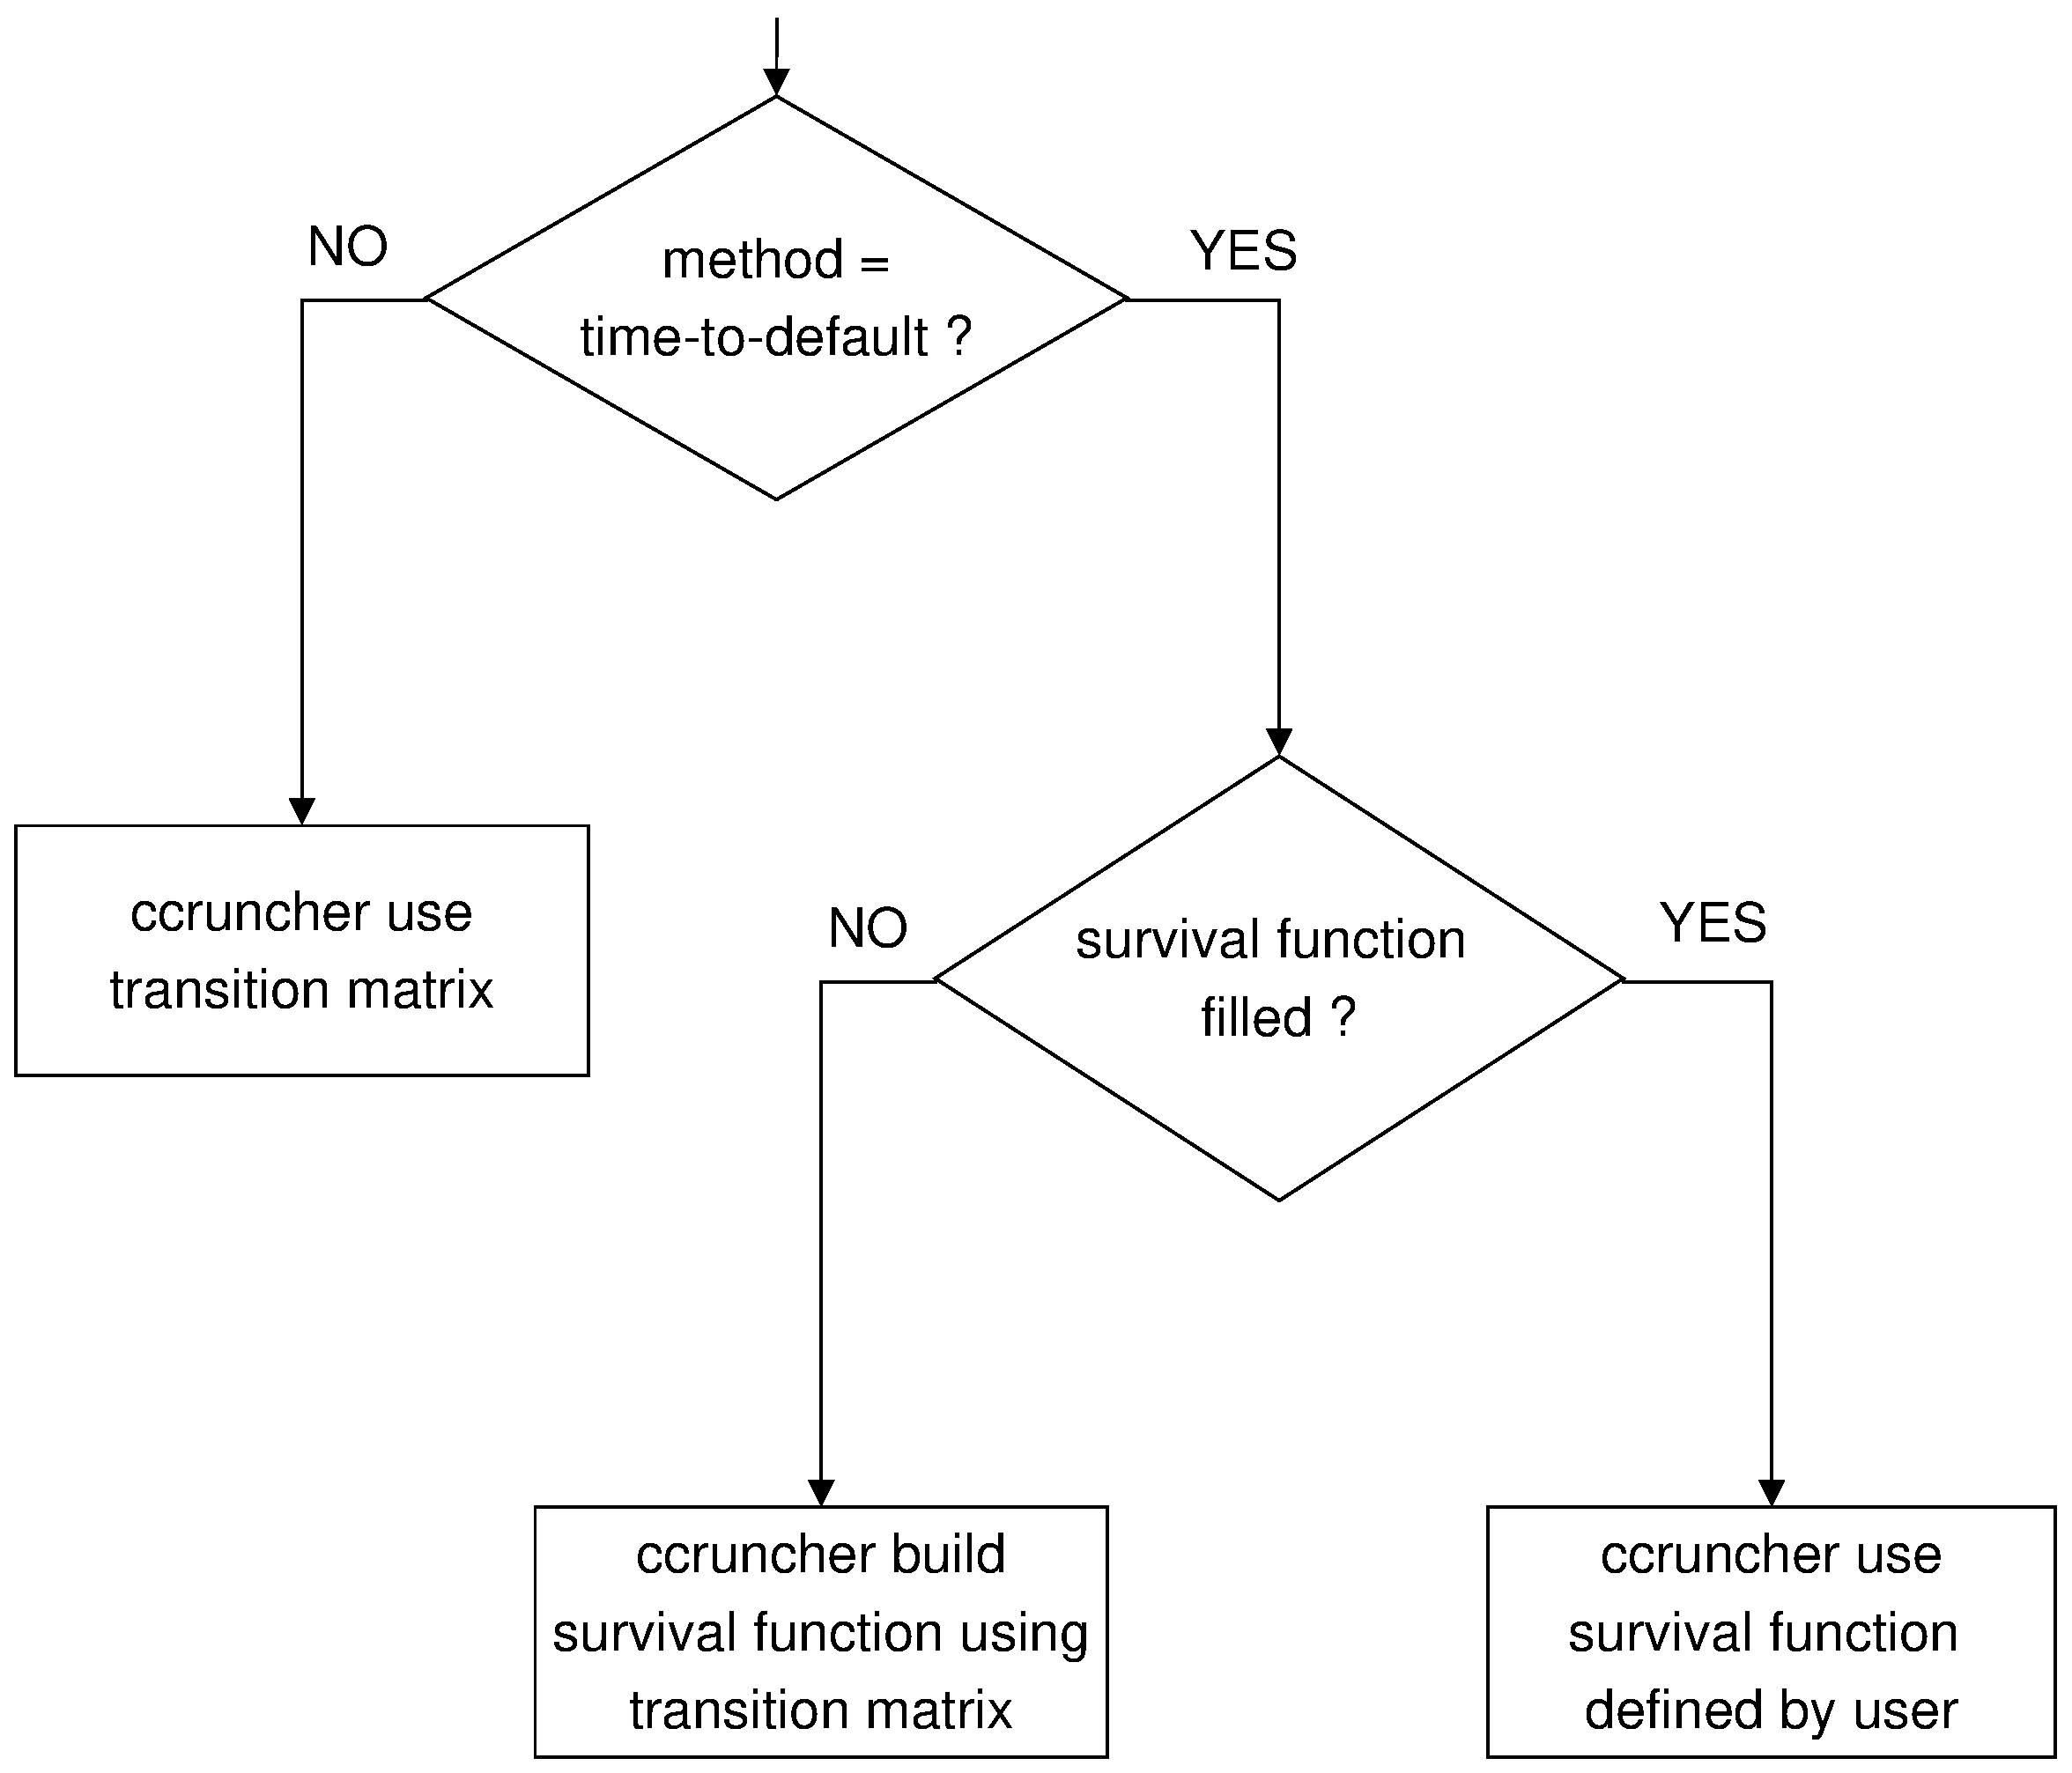
\includegraphics[width=10cm,angle=0]{./images/decisiontree1.eps}
\caption{Decisi\'on en funci\'on del m\'etodo}
\label{decisiontree1}
\end{center}
\end{figure}

precalculo de los valores en los nodos


\section{Proceso de agregaci\'on}

TODO: descripcion de los agregadores y metodo usado para evitar recalculo 
de los activos en cada simulacion + Agregaci\'on de productos


\section{Dimensiones del problema}

TODO: Estimaciones de uso de memoria, estimaci\'on del numero de operaciones,
estimacion del tiempo de computo


\section{Convergencia de la soluci\'on}

TODO: N\'umero de iteraciones necesarias, aceleraci\'on de la convergencia
usando metodolog\'ia antithetic

convergencia media, varianza, var (estimadores, graficos, etc.)
